\documentclass[12pt,a4paper]{ctexart}

\usepackage{amsmath,amssymb}
\usepackage[margin=2.5cm]{geometry}
\usepackage{booktabs}
\usepackage{graphicx}
\usepackage{array}
\usepackage{caption}
\usepackage{float}
\usepackage{enumitem}
\usepackage{hyperref}
\usepackage{multirow}

\captionsetup{font=small,labelfont=bf}
\setlength{\parindent}{2em}
\allowdisplaybreaks
\graphicspath{{../figures/}}
\hypersetup{colorlinks=true,linkcolor=black,citecolor=black,urlcolor=blue}

\newcommand{\dd}{\mathrm{d}}

\begin{document}

% ================= 摘要 =================
\begin{center}
{\Large\bfseries 药材预热平衡阶段温度与水分浓度分布的数值求解}\\[6pt]
{\normalsize ——基于 Euler 显式与 Crank--Nicolson 隐式格式的径向一维模型}
\end{center}

\begin{abstract}
\noindent 药材干燥是中药材品质控制的关键工序，预热平衡阶段内部温度与水分浓度的时空演化规律直接影响后续恒温干燥的工艺设定。本文针对给定半径 $2$ cm、长 $25$ cm 的圆柱形药材，建立径向一维非稳态热质传递模型，求解前 $30$ min 内药材内部温度与含水率的时空分布。

对于问题一，首先依据长径比与特征扩散长度将问题降维为无限长圆柱的径向一维问题，建立热传导方程与水分扩散方程；其次\textbf{完整实现 Euler 显式（向前 Euler）方法}，把径向节点严格划分为\textbf{中心点、内部点、边界点}三类分别离散：中心点用 L'H\^opital 法则消去 $1/r$ 奇异项并结合轴对称条件，内部点用柱坐标守恒型中心差分，边界点用 Robin 对流边界的半控制体积离散；显式格式逐点推进、无需解线性方程组、对变扩散系数 $D(C)$ 亦无需迭代，但受抛物型 CFL 稳定条件 $Fo=\alpha\Delta t/\Delta r^2\le0.41$ 限制（柱坐标下略严于笛卡尔情形的 $1/2$）。在此基础上\textbf{引入 Crank--Nicolson 隐式格式与 Thomas 追赶法}，将时间精度由一阶提升至二阶、并解除 CFL 限制实现无条件稳定，三对角方程组由 Thomas 追赶法以 $O(N)$ 复杂度求解。

结果表明，热扩散系数约为水分扩散系数的 $34$ 倍（$\mathrm{Fo}_T=0.760$、$\mathrm{Fo}_C=0.0222$），$1800$ s 时温度场已整体抬升（中心 $33.575$ $^\circ$C、表面 $36.785$ $^\circ$C、径向温差 $3.21$ $^\circ$C），而水分场仅外层约 $1.5$ cm 壳体失水（表面含水率降幅 $40.70\%$、体积平均降幅 $10.11\%$）。数值验证表明：Euler 显式与 CN 在 $\Delta t=1$ s 下四位小数一致；CN 格式可放大时间步 $300$ 倍而不失稳，显式格式在 $Fo>0.41$ 时迅速发散。本文结论可为预热平衡阶段的工艺时间窗口提供定量依据。

\noindent\textbf{关键词：}径向一维热质传递；Euler 显式方法；Crank--Nicolson 格式；Thomas 追赶法；CFL 稳定性
\end{abstract}

\tableofcontents
\newpage

% ================= 一、引言 =================
\section{引言}
\subsection{问题背景}
干燥是决定中药材成品品质的关键工序之一。热风烘干通过调控烘房温湿环境完成药材干燥，其工艺参数选取不当会导致干燥效率低、能耗高、成品品质不稳定。传统试验优化模式成本高、周期长，亟需借助数理分析与数值仿真得到干燥规律。

预热平衡阶段是干燥的第一阶段，药材被烘房加热、内部温度逐步趋近环境、表层水分开始向表面迁移并汽化。该阶段内部温度与含水率的分布直接决定了后续恒温干燥阶段的初始状态与工艺时点的选取，因此需要求解一个含变系数、带对流边界的瞬态热质传递问题。

\subsection{问题重述}
\textbf{问题1}：某中药材形状大致呈圆柱形，长 $25$ cm、半径 $2$ cm。烘干开始时药材温度为 $28$ $^\circ$C、水分浓度（干基含水率）为 $2.55$ kg/kg，烘房温度与水分浓度随时间变化见附件 1。请建立预热平衡阶段药材温度和水分浓度变化规律的数学模型（相关参数见附录 2），在论文中按表 1、表 2 格式给出 $100,300,600,900,1200,1500,1800$ s、到药材中心距离 $0,0.5,1,1.5,2$ cm 处的温度与水分浓度，并将 $1800$ s 内每隔 $1$ s、每隔 $0.1$ cm 的完整结果保存到 \texttt{result1.xlsx}。所有结果保留四位小数。

% ================= 二、总体分析 =================
\section{总体分析}
本题的本质是求解无限长圆柱内的\textbf{径向一维非稳态热质传递}问题。热量由烘房经表面对流换热带入药材内部，水分由内部向表面迁移并经表面汽化进入烘房。二者在几何上共用同一圆柱体，在时间上共用同一环境条件记录，但在题设附录 2 的参数体系下，热方程不含水分项（未给出汽化潜热），故热与质之间为\textbf{单向耦合}，两方程可按"先热后质"的顺序逐时间步求解。

数值方法的选择是本题的核心。本文采用"先显式、后隐式"的递进策略：首先\textbf{完整实现 Euler 显式方法}，把径向节点分为中心点、内部点、边界点三类分别离散，其优点是逐点推进、无需解线性方程组、对非线性 $D(C)$ 无需迭代，缺点是受 CFL 稳定条件限制、时间只有一阶精度；在此基础上\textbf{引入 Crank--Nicolson 隐式格式与 Thomas 追赶法}，用无条件稳定性换取时间二阶精度与更大的时间步。这一递进既能清楚呈现差分格式的构造逻辑，又能说明隐式格式相对显式格式的定量收益。

% ================= 三、模型假设 =================
\section{模型假设}
为简化问题，本文做出以下假设：
\begin{itemize}
\item \textbf{假设 1（几何）}：药材为均质、各向同性的无限长圆柱，温度与水分浓度仅沿径向变化。
\item \textbf{假设 2（物性）}：药材密度 $\rho$、比热容 $c_p$、导热系数 $k$ 在所考察温度与含水率范围内取常值。
\item \textbf{假设 3（初始状态）}：药材内部初始温度与含水率均匀，分别为 $T_0=28$ $^\circ$C、$C_0=2.55$ kg/kg（干基）。
\item \textbf{假设 4（边界）}：药材表面与烘房环境之间的换热与传质均服从牛顿冷却定律形式，即通量与表面—环境之差的一次方成正比。
\item \textbf{假设 5（无内源）}：药材内部无相变潜热释放、无化学放热、无水分生成。这是本问最主要的简化——干燥中水分汽化所需潜热由药材自身供给，因题设未给出汽化潜热，该项被略去。
\item \textbf{假设 6（扩散形式）}：水分迁移服从 Fick 定律，有效扩散系数 $D$ 仅依赖局部含水率 $C$。
\end{itemize}

% ================= 四、符号说明 =================
\section{符号说明}
本文使用的主要符号及其含义如表 \ref{tab:symbol} 所示。

\begin{table}[H]
\centering
\caption{符号说明}
\label{tab:symbol}
\resizebox{\textwidth}{!}{%
\begin{tabular}{llll}
\toprule
符号 & 含义 & 单位 & 取值/来源 \\
\midrule
$r$ & 到药材中心的径向距离 & m & $0\le r\le R$ \\
$t$ & 时间 & s & $0\le t\le 1800$ \\
$R$ & 药材半径 & m & $0.02$ \\
$L$ & 药材长度 & m & $0.25$ \\
$T(r,t)$ & 药材内部温度 & $^\circ$C & 待求 \\
$C(r,t)$ & 药材含水率（干基） & kg/kg & 待求 \\
$T_\infty(t)$ & 烘房环境温度 & $^\circ$C & 附件 1 \\
$C_\infty(t)$ & 烘房环境水分浓度 & kg/kg & 附件 1 \\
$\rho$ & 药材密度 & kg/m$^3$ & 820 \\
$c_p$ & 药材比热容 & J/(kg$\cdot$K) & 2600 \\
$k$ & 导热系数 & W/(m$\cdot$K) & 0.36 \\
$h$ & 对流换热系数 & W/(m$^2\cdot$K) & 25 \\
$h_m$ & 对流传质系数 & m/s & $8\times10^{-7}$ \\
$\alpha$ & 热扩散系数 $\alpha=k/(\rho c_p)$ & m$^2$/s & $1.689\times10^{-7}$ \\
$D(C)$ & 水分有效扩散系数 & m$^2$/s & $7\times10^{-9}e^{-0.89/C}$ \\
$\Delta r$ & 径向网格步长 & m & $10^{-3}$ \\
$\Delta t$ & 时间步长 & s & 1 \\
$N$ & 径向网格数 & — & 20 \\
$Fo$ & Fourier 数 $Fo=\alpha\Delta t/\Delta r^2$ & — & 0.169 \\
\bottomrule
\end{tabular}}
\end{table}

% ================= 五、模型的建立与求解 =================
\section{模型的建立与求解}
\subsection{问题一的模型的建立和求解}

\subsubsection{具体分析}
问题一要求给出预热平衡阶段药材内部温度与水分浓度的时空分布，属于\textbf{机理分析}类问题。本问采用\textbf{有限差分法}进行求解：首先建立径向一维热质传递的偏微分方程模型，接着用 Euler 显式方法完成初步求解，再用 Crank--Nicolson 隐式格式改进时间精度并解除稳定性限制，最后通过 Thomas 追赶法高效求解三对角方程组。

\textbf{降维依据。} 药材为半径 $R=2$ cm、长 $L=25$ cm 的圆柱，长径比 $L/(2R)=6.25$。比较特征扩散长度与几何尺寸：$30$ min 内热扩散长度 $\sqrt{\alpha t}=1.74$ cm，占半长 $12.5$ cm 的 $13.9\%$、占半径的 $87\%$；水分扩散长度 $\sqrt{D(C_0)t}=0.30$ cm，占半长 $2.4\%$、占半径的 $15\%$。热量的径向扩散长度已与半径同量级，径向梯度不可忽略；而两者相对半长都较小，轴向中段一维性成立。故将问题简化为\textbf{径向一维}。两端面面积仅占总表面积的 $R/L=8\%$，进一步支持忽略轴向。

具体分析流程如图 \ref{fig:flow} 所示。

\begin{figure}[H]
\centering
\fbox{\parbox{0.92\textwidth}{\centering
\begin{tabular}{c c c c c c c c c}
读取附件 & $\rightarrow$ & 建立控制方程 & $\rightarrow$ & 定解条件 & $\rightarrow$ & 节点分类离散 & $\rightarrow$ & 输出结果 \\
\multicolumn{9}{c}{Euler 显式（中心/内部/边界三类节点）$\;\rightarrow\;$ Crank--Nicolson + Thomas 追赶法}
\end{tabular}}}
\caption{问题一分析流程图}
\label{fig:flow}
\end{figure}

\subsubsection{模型准备}
\textbf{数据来源与预处理。} 环境条件 $T_\infty(t),C_\infty(t)$ 来自附件 1，以 $60$ s 为间隔给出 $241$ 个离散点（覆盖 $0\sim14400$ s）。本计算在 $60$ s 整数倍时刻取节点值，其余时刻按\textbf{分段线性插值}取值（区间外按端点常数延拓）。该项引入的误差为 $O(\Delta t_{\text{采样}}^2 T_\infty'')$，小于空间离散误差，不构成主要误差来源。

\textbf{算法选型。} 求解抛物型偏微分方程（热质传递）的常用数值方法包括 Euler 显式、Crank--Nicolson 隐式、向后 Euler 等。表 \ref{tab:algo} 从稳定性、时间精度、实现复杂度三方面进行对比。

\begin{table}[H]
\centering
\caption{候选数值格式对比}
\label{tab:algo}
\begin{tabular}{lccc}
\toprule
数值格式 & 稳定性 & 时间精度 & 实现复杂度 \\
\midrule
Euler 显式（$\theta=0$） & 条件稳定（$Fo\le0.41$） & 一阶 & 低（无线性方程组） \\
向后 Euler（$\theta=1$） & 无条件稳定 & 一阶 & 中（需解三对角） \\
Crank--Nicolson（$\theta=1/2$） & 无条件稳定 & 二阶 & 中（需解三对角） \\
\bottomrule
\end{tabular}
\end{table}

通过对比，本文采用"先显式后隐式"的策略：先以 Euler 显式完成求解并验证三类节点离散的正确性，再以 Crank--Nicolson 格式获得时间二阶、无条件稳定的最终结果。三对角方程组统一由 Thomas 追赶法求解。

\subsubsection{模型建立}
\paragraph{控制方程。} 取半径为 $r$、厚度 $\dd r$ 的环形控制体（单位长度），其体积为 $2\pi r\,\dd r$。分别对控制体作能量守恒与水分质量守恒。

\textbf{能量守恒}：控制体内焓的时间变化率等于两侧径向净导入的导热热流，
\begin{equation}
\rho c_p\frac{\partial T}{\partial t}=\frac{1}{r}\frac{\partial}{\partial r}\!\left(k\,r\frac{\partial T}{\partial r}\right)
\label{eq:heat}
\end{equation}

\textbf{水分质量守恒}：控制体内水分的质量变化率等于两侧径向净导入的扩散通量，
\begin{equation}
\frac{\partial C}{\partial t}=\frac{1}{r}\frac{\partial}{\partial r}\!\left(D(C)\,r\frac{\partial C}{\partial r}\right)
\label{eq:mass}
\end{equation}

其中 $D(C)=7\times10^{-9}e^{-0.89/C}$ 使式 \eqref{eq:mass} 成为拟线性方程，是数值处理的难点。两方程具有统一形式
\begin{equation}
\frac{\partial u}{\partial t}=\frac{1}{r}\frac{\partial}{\partial r}\!\left(\beta\,r\frac{\partial u}{\partial r}\right),\qquad
\beta=\alpha\ \text{（热）},\ \beta=D(C)\ \text{（质）}
\label{eq:unified}
\end{equation}

\paragraph{定解条件。}
\textbf{初始条件}：
\begin{equation}
T(r,0)=28\ ^\circ\mathrm{C},\qquad C(r,0)=2.55\ \mathrm{kg/kg}
\label{eq:init}
\end{equation}

\textbf{中心对称条件}（$r=0$，由几何轴对称性，中心处无径向通量）：
\begin{equation}
\left.\frac{\partial T}{\partial r}\right|_{r=0}=0,\qquad
\left.\frac{\partial C}{\partial r}\right|_{r=0}=0
\label{eq:center}
\end{equation}

\textbf{表面对流边界}（$r=R$，Robin 条件）：热侧由题设附录给出，
\begin{equation}
-k\left.\frac{\partial T}{\partial r}\right|_{R}=h\left[T(R,t)-T_\infty(t)\right]
\label{eq:robinT}
\end{equation}

水分侧由传质类比补全：表面水分汽化通量与表面—环境水分浓度差成正比，
\begin{equation}
-D(C)\left.\frac{\partial C}{\partial r}\right|_{R}=h_m\left[C(R,t)-C_\infty(t)\right]
\label{eq:robinC}
\end{equation}

\paragraph{无量纲特征量。} 求解前先估算特征数，以判断格式刚度与边界控制机制，如表 \ref{tab:charnum} 所示。

\begin{table}[H]
\centering
\caption{无量纲特征量}
\label{tab:charnum}
\resizebox{\textwidth}{!}{%
\begin{tabular}{llcl}
\toprule
特征量 & 定义 & 数值 & 含义 \\
\midrule
热 Biot 数 & $\mathrm{Bi}_T=hR/k$ & $1.39$ & 径向温度梯度不可忽略 \\
质 Biot 数 & $\mathrm{Bi}_m=h_mR/D(C_0)$ & $3.24$ & 过程由内部扩散控制 \\
热 Fourier 数 & $\mathrm{Fo}_T=\alpha t/R^2$ & $0.760$ & 30 min 内热量已穿透至中心 \\
质 Fourier 数 & $\mathrm{Fo}_C=D(C_0)t/R^2$ & $0.0222$ & 30 min 内水分迁移刚起步 \\
特征时间比 & $\alpha/D(C_0)$ & $34.2$ & 热响应比质响应快 34 倍 \\
\bottomrule
\end{tabular}}
\end{table}

$\mathrm{Fo}_T$ 与 $\mathrm{Fo}_C$ 相差 $34$ 倍，预示温度场将达到近平衡而水分场仅表面响应。

\subsubsection{模型求解}
本节先\textbf{完整实现 Euler 显式方法}，把径向节点分为\textbf{中心点、内部点、边界点}三类分别离散；随后\textbf{引入 Crank--Nicolson 隐式格式与 Thomas 追赶法}，作为时间精度与稳定性的升级。

\paragraph{第一步：Euler 显式方法的节点分类离散。}
对式 \eqref{eq:unified} 作时间向前 Euler 离散，得
\begin{equation}
\frac{u^{n+1}_j-u^{n}_j}{\Delta t}=\big(L_h u^n\big)_j
\qquad\Longleftrightarrow\qquad
u^{n+1}_j=u^{n}_j+\Delta t\,\big(L_h u^n\big)_j
\label{eq:explicit}
\end{equation}
其中 $L_h$ 为空间差分算子，右端全部取已知的第 $n$ 时刻值。空间离散按节点位置分为三类。

\textbf{(i) 中心点 $j=0$。} 式 \eqref{eq:unified} 右端在 $r\to0$ 时呈 $\tfrac00$ 型不定式，用 L'H\^opital 法则并结合对称条件 \eqref{eq:center}：
\begin{equation}
\lim_{r\to0}\frac{1}{r}\frac{\partial}{\partial r}\!\left(\beta\,r\frac{\partial u}{\partial r}\right)
=2\beta\left.\frac{\partial^2 u}{\partial r^2}\right|_{r=0}
\label{eq:lhopital}
\end{equation}
再以对称虚拟点 $u_{-1}=u_1$ 作二阶中心差分 $\partial^2u/\partial r^2|_0=2(u_1-u_0)/\Delta r^2$，得中心节点离散
\begin{equation}
\frac{\dd T}{\dd t}\Big|_0=\frac{4\alpha}{\Delta r^2}(T_1-T_0),\qquad
\frac{\dd C}{\dd t}\Big|_0=\frac{4D_{1/2}}{\Delta r^2}(C_1-C_0)
\label{eq:center_disc}
\end{equation}
显式更新为
\begin{equation}
T_0^{n+1}=T_0^{n}+\Delta t\cdot\frac{4\alpha}{\Delta r^2}\big(T_1^n-T_0^n\big)
\label{eq:center_explicit}
\end{equation}

\textbf{(ii) 内部点 $1\le j\le N-1$。} 对节点 $r_j=j\Delta r$ 的控制体 $[r_{j-1/2},r_{j+1/2}]$ 作守恒积分（而非直接差分），得柱坐标守恒型中心差分
\begin{equation}
\frac{\dd u_j}{\dd t}=\frac{1}{r_j\Delta r^2}\Big[\beta_{j-\frac12}r_{j-\frac12}(u_{j-1}-u_j)+\beta_{j+\frac12}r_{j+\frac12}(u_{j+1}-u_j)\Big]
\label{eq:interior_disc}
\end{equation}
其中界面扩散系数取算术平均 $\beta_{j+1/2}=(\beta_j+\beta_{j+1})/2$。对热方程 $\beta\equiv\alpha$，$r_{j\pm1/2}/r_j=(j\pm1/2)/j$，显式更新为
\begin{equation}
T_j^{n+1}=T_j^{n}+\Delta t\cdot\frac{\alpha}{\Delta r^2}
\left[\frac{j-\tfrac12}{j}\,T_{j-1}^n-2\,T_j^n+\frac{j+\tfrac12}{j}\,T_{j+1}^n\right]
\label{eq:interior_explicit}
\end{equation}

\textbf{(iii) 边界点 $j=N$。} 取表面节点控制体 $[r_{N-1/2},R]$（半控制体，外侧即物理表面），其径向权重为
\begin{equation}
V_N=\int_{r_{N-1/2}}^{R}r\,\dd r=\frac{R\,\Delta r}{2}-\frac{\Delta r^2}{8}
\label{eq:VN}
\end{equation}
在该控制体上积分式 \eqref{eq:unified}，内侧通量用中心差分、外侧通量直接由 Robin 条件 \eqref{eq:robinT} 代入（不引入虚拟节点）：
\begin{equation}
\frac{\dd T_N}{\dd t}=
\frac{\alpha\,r_{N-\frac12}}{V_N\,\Delta r}(T_{N-1}-T_N)
-\frac{R\,h}{\rho c_p\,V_N}\big[T_N-T_\infty\big]
\label{eq:boundary_disc}
\end{equation}
水分侧形式相同，仅将 $\alpha\to D_{N-1/2}$、$h/(\rho c_p)\to h_m$。显式更新为
\begin{equation}
T_N^{n+1}=T_N^{n}+\Delta t\left[
\frac{\alpha\,r_{N-\frac12}}{V_N\,\Delta r}(T_{N-1}^n-T_N^n)
-\frac{R\,h}{\rho c_p\,V_N}\big(T_N^n-T_\infty^n\big)\right]
\label{eq:boundary_explicit}
\end{equation}

显式方法的关键优势在于：\textbf{右端全部使用已知的第 $n$ 时刻值}，逐点直接更新，无需解线性方程组；对拟线性方程 \eqref{eq:mass}，$D(C)$ 直接取 $C^n$ 计算（滞后取当前时刻），\textbf{无需 Picard 迭代}。

\textbf{显式方法的稳定性（CFL 条件）。} 显式格式要求时间步满足抛物型稳定性条件。对柱坐标扩散算子，中心节点含 $4\alpha/\Delta r^2$ 系数、边界含 Robin 对流项，其最大特征值模 $\lambda_{\max}=0.8176$ s$^{-1}$（略大于笛卡尔情形的 $4\alpha/\Delta r^2=0.6754$ s$^{-1}$），故稳定条件为
\begin{equation}
\Delta t\le\frac{2}{\lambda_{\max}}=2.446\ \text{s}
\qquad\Longleftrightarrow\qquad
Fo=\frac{\alpha\Delta t}{\Delta r^2}\le 0.413
\label{eq:cfl}
\end{equation}
即柱坐标下显式格式的稳定边界 $Fo\le0.41$，略严于笛卡尔一维的 $Fo\le1/2$。本文取 $\Delta t=1$ s（$Fo=0.169$），既满足稳定条件又使时间误差远小于空间误差。

\paragraph{第二步：Crank--Nicolson 隐式格式与 Thomas 追赶法。}
将式 \eqref{eq:center_disc}、\eqref{eq:interior_disc}、\eqref{eq:boundary_disc} 统一写为算子形式 $\dd u/\dd t=Lu+s$，其中源项 $s_j=\delta_{jN}\,g\,u_\infty$ 仅表面节点非零。取 $\theta$ 格式
\begin{equation}
\big(I-\theta\Delta t\,L\big)u^{n+1}=\big(I+(1-\theta)\Delta t\,L\big)u^{n}
+\Delta t\big[\theta\,s^{n+1}+(1-\theta)\,s^{n}\big]
\label{eq:theta}
\end{equation}
$\theta=1/2$ 即 Crank--Nicolson；$\theta=1$ 为向后 Euler；$\theta=0$ 退化为式 \eqref{eq:explicit} 的显式格式。式 \eqref{eq:theta} 左端为三对角矩阵，用 \textbf{Thomas 追赶法}求解：先前向消元求系数 $\psi_i,\phi_i$，再后向回代，计算复杂度 $O(N)$、存储 $O(N)$。

\textbf{无条件稳定性。} 对特征值 $\lambda\ge0$，$\theta$ 格式的增长因子为
\begin{equation}
G(\lambda)=\frac{1+(1-\theta)\lambda\Delta t}{1+\theta\lambda\Delta t},
\qquad
|G(\lambda)|\le1\ \ \text{对任意}\ \Delta t>0\ \ (\theta\ge\tfrac12)
\label{eq:growth}
\end{equation}
故 CN 格式不受式 \eqref{eq:cfl} 的限制，时间步可按精度需要而非稳定性需要选取。

\textbf{$D(C)$ 的滞后迭代。} 式 \eqref{eq:mass} 因 $D=D(C)$ 而拟线性。在每个时间步内令扩散系数取上一轮迭代的浓度（滞后），并\textbf{区分新旧时间层的算子}：
\begin{equation}
\frac{u^{n+1}-u^{n}}{\Delta t}
=\frac12\Big[L(D^n)u^{n}+L(D^{n+1})u^{n+1}\Big]
\label{eq:cn_varc}
\end{equation}
即旧时间层用旧系数 $D^n$、新时间层用新系数 $D^{n+1}$。若两个时间层都套用新算子，局部截断误差中将出现 $O(\Delta t)$ 的系数错配项，使 CN 退化为时间一阶。迭代至 $\|C^{(k+1)}-C^{(k)}\|_\infty<10^{-10}$（实测 2 次收敛）。

\paragraph{求解流程。} 每个时间步内：① 由附件 1 取本步 $T_\infty(t),C_\infty(t)$（分段线性插值）；② 求解温度方程（常系数，一次 Thomas 求解）；③ 以 $C^n$ 组装旧算子、以当前迭代值组装新算子，作 Thomas 求解得 $C^{(k+1)}$；④ 检验收敛，未收敛返回第 ③ 步。

\paragraph{结果。} 取 $N=20$（$\Delta r=0.1$ cm）、$\Delta t=1$ s，算至 $t=1800$ s。Euler 显式与 CN 在 $\Delta t=1$ s 下终态最大差为 $|dT|=5.02\times10^{-3}$ $^\circ$C、$|dC|=8.74\times10^{-5}$ kg/kg，二者\textbf{四位小数一致}；最终结果取时间二阶的 CN 值。表 \ref{tab:T}、\ref{tab:C} 为要求位置与时刻的结果（完整逐秒、逐 0.1 cm 数据见 \texttt{result1.xlsx}）。

\begin{table}[H]
\centering
\caption{表 1　30 分钟内药材的温度（$^\circ$C）}
\label{tab:T}
\begin{tabular}{lccccc}
\toprule
时间/s & 0 cm（中心） & 0.5 cm & 1.0 cm & 1.5 cm & 2.0 cm（表面） \\
\midrule
100  & 28.0001 & 28.0004 & 28.0041 & 28.0326 & 28.1786 \\
300  & 28.0411 & 28.0638 & 28.1514 & 28.3676 & 28.8469 \\
600  & 28.4537 & 28.5363 & 28.8039 & 29.3153 & 30.1640 \\
900  & 29.3245 & 29.4584 & 29.8753 & 30.6156 & 31.7297 \\
1200 & 30.5428 & 30.7098 & 31.2222 & 32.1121 & 33.4269 \\
1500 & 31.9957 & 32.1867 & 32.7658 & 33.7460 & 35.1204 \\
1800 & 33.5752 & 33.7719 & 34.3640 & 35.3619 & 36.7853 \\
\bottomrule
\end{tabular}
\end{table}

\begin{table}[H]
\centering
\caption{表 2　30 分钟内药材的水分浓度（kg/kg，干基）}
\label{tab:C}
\begin{tabular}{lccccc}
\toprule
时间/s & 0 cm（中心） & 0.5 cm & 1.0 cm & 1.5 cm & 2.0 cm（表面） \\
\midrule
100  & 2.5500 & 2.5500 & 2.5500 & 2.5500 & 2.2880 \\
300  & 2.5500 & 2.5500 & 2.5500 & 2.5486 & 2.0661 \\
600  & 2.5500 & 2.5500 & 2.5500 & 2.5342 & 1.8846 \\
900  & 2.5500 & 2.5500 & 2.5495 & 2.5041 & 1.7596 \\
1200 & 2.5500 & 2.5500 & 2.5478 & 2.4647 & 1.6619 \\
1500 & 2.5500 & 2.5499 & 2.5440 & 2.4212 & 1.5812 \\
1800 & 2.5500 & 2.5496 & 2.5376 & 2.3763 & 1.5120 \\
\bottomrule
\end{tabular}
\end{table}

\paragraph{结果分析。}
图 \ref{fig:profile} 给出 $t=100,300,900,1800$ s 的径向剖面。温度剖面（图 \ref{fig:profile}a）在各时刻均呈中心低、表面高的单调上升形态，$1800$ s 时中心 $33.575$ $^\circ$C、表面 $36.785$ $^\circ$C，径向温差 $3.21$ $^\circ$C；此时环境温度 $T_\infty(1800)=41.513$ $^\circ$C，径向温差占"环境—中心"总位差 $7.94$ $^\circ$C 的 $40.4\%$，中心明显滞后、过程未进入拟稳态。水分为完全不同的形态（图 \ref{fig:profile}b）：$r\lesssim1$ cm 区域几乎保持初值，外侧形成陡峭浓度边界层并随时间向内推进。

$1800$ s 时表面含水率由 $2.55$ 降至 $1.5120$ kg/kg，表面降幅 $40.70\%$；而体积加权平均含水率仅由 $2.5500$ 降至 $2.2921$，整体失水 $10.11\%$。失水高度集中于外层壳体，若按整体平均含水率判断干燥进度会显著低估表层干裂风险。

\begin{figure}[H]
\centering
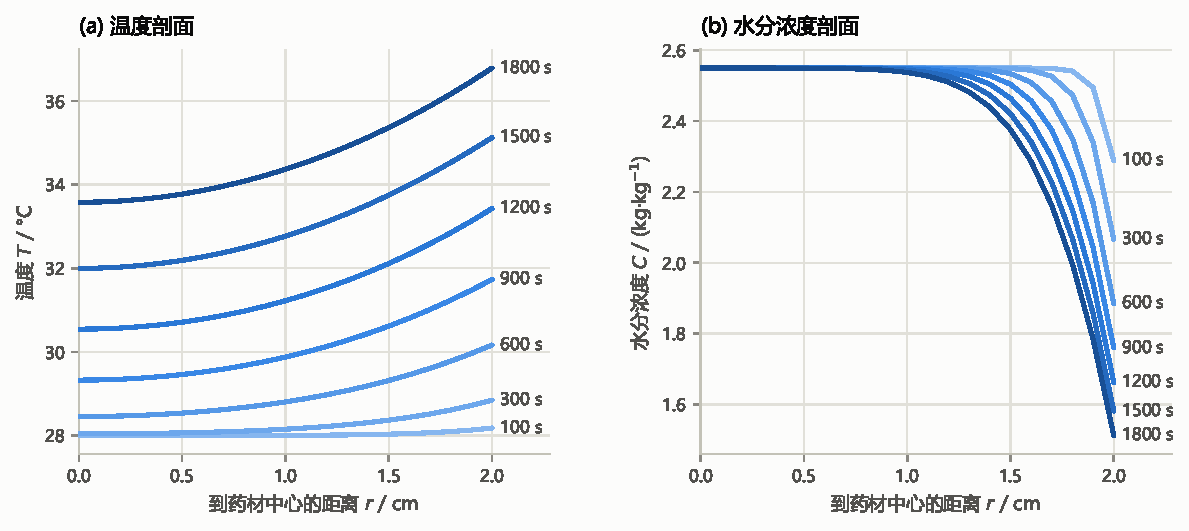
\includegraphics[width=0.96\textwidth]{fig1_预热平衡阶段剖面.pdf}
\caption{预热平衡阶段药材内部温度（a）与水分浓度（b）的径向剖面}
\label{fig:profile}
\end{figure}

% ================= 六、模型检验与分析 =================
\section{模型检验与分析}
为验证模型与数值格式的有效性，进行以下检验。

\subsection{误差分析}
\textbf{（1）与独立解析解对比。} 构造无限长圆柱、常环境温度对流边界下的解析解（分离变量级数解，Bessel 函数展开，取 60 项）作为基准。取 $T_\infty=50$ $^\circ$C、$N=160$、$\Delta t=0.05$ s，数值解与解析解的最大偏差在 $10^{-5}$ $^\circ$C 量级（$t=300$ s 时 $5.31\times10^{-5}$ $^\circ$C），相对误差小于 $10^{-6}$。该算例同时检验了中心 L'H\^opital 处理与表面 Robin 离散的正确性。

\textbf{（2）空间与时间收敛阶。} 空间方向（固定 $\Delta t=0.02$ s，以 $N=640$ 为参考解）观测阶为 $2.01,2.02,2.07$，温度与浓度场均呈\textbf{二阶收敛}；时间方向（固定 $N=40$）CN 格式观测阶为 $2.00$，呈\textbf{时间二阶}；而 Euler 显式格式时间收敛阶为 $1.00$（一阶）。这正是引入 CN 格式的精度收益。

\textbf{（3）全局守恒回代。} 以守恒权重 $w_0=\Delta r^2/8$、$w_j=r_j\Delta r$、$w_N=R\Delta r/2-\Delta r^2/8$ 作加权和，$\sum_j w_j=\Delta r^2/8$ 精确等于圆柱截面积积分，且所有内部界面通量两两相消，仅余表面项。全局热平衡与质量平衡的相对偏差分别为 $2.93\times10^{-14}$、$1.94\times10^{-14}$，在浮点舍入水平，说明离散守恒为恒等式。

\subsection{灵敏度分析}
\textbf{（1）稳定性对比。} 环境恒为 $T_\infty=50$ $^\circ$C（精确解恒有 $T\le50$ $^\circ$C），任何超界取值均为非物理放大。Crank--Nicolson 格式在 $\Delta t$ 放大至 $300$ s（$300$ 倍）时表面温度仅变化 $1.1$ $^\circ$C，验证\textbf{无条件稳定}；Euler 显式格式在 $Fo=0.405$（$\Delta t=2.4$ s）时有界，而在 $Fo=0.422$（$\Delta t=2.5$ s）时即发散至 $10^6$ 量级，与式 \eqref{eq:cfl} 的临界值 $Fo_{\text{crit}}=0.413$ 精确一致。这定量说明了"由显式升级为 CN"的直接收益：时间步可放大两个数量级而不失稳。

\begin{table}[H]
\centering
\caption{显式与隐式格式的稳定性对比（$N=20$，$t_{\text{end}}=1800$ s）}
\label{tab:stability}
\resizebox{\textwidth}{!}{%
\begin{tabular}{lccccc}
\toprule
格式 & $\Delta t$ / s & $Fo=\alpha\Delta t/\Delta r^2$ & $T_{\max}$ / $^\circ$C & 物理有界 \\
\midrule
\multirow{3}{*}{Euler 显式} & 1.0 & 0.169 & $4.6642\times10^{1}$ & $\checkmark$ \\
 & 2.4 & 0.405 & $4.6645\times10^{1}$ & $\checkmark$ \\
 & 2.5 & 0.422 & $1.1553\times10^{6}$ & $\times$ \\
\midrule
\multirow{3}{*}{Crank--Nicolson} & 10 & — & $46.6396$ & $\checkmark$ \\
 & 60 & — & $46.6264$ & $\checkmark$ \\
 & 300 & — & $46.4007$ & $\checkmark$ \\
\bottomrule
\end{tabular}}
\end{table}

\textbf{（2）热物性参数敏感性。} 热扩散系数 $\alpha$ 变化 $\pm20\%$ 使中心温度变化约 $\mp0.6$ $^\circ$C、表面温度仅约 $\pm0.2$ $^\circ$C，且符号相反——$\alpha$ 越小表面热量越难向内传导，表面温度越接近环境温度。故热物性不确定性主要影响内部温度而非表面温度。

\textbf{（3）扩散系数非线性影响。} 将 $D$ 强制取常值 $D(C_0)$ 重算作为基线，常系数近似高估整体失水量 $1.25\%$（表面浓度高估 $2.72\%$）。方向与 $D(C)$ 的负反馈（自减速）机制一致，但幅度小，因 30 min 内浓度变化集中于表层。

% ================= 七、模型的评价 =================
\section{模型的评价}
\subsection{模型的优点}
\begin{itemize}
\item \textbf{优点 1}：数值方法递进清晰，先以 Euler 显式方法完整呈现中心点、内部点、边界点三类节点的离散构造，再引入 Crank--Nicolson 与 Thomas 追赶法，使格式的物理含义与升级动机一目了然。
\item \textbf{优点 2}：中心点用 L'H\^opital 法则消去 $1/r$ 奇异性、边界点用半控制体积精确平衡，二者均保持二阶精度与离散守恒（守恒偏差 $10^{-14}$ 量级）。
\item \textbf{优点 3}：格式对比量化，显式方法的 CFL 边界（$Fo_{\text{crit}}=0.413$）由特征值精确导出并与数值实验一致，CN 的无条件稳定性收益得到定量验证。
\end{itemize}
\subsection{模型的缺点}
\begin{itemize}
\item \textbf{缺点 1}：未计蒸发潜热（题设未给出汽化潜热），热方程无汇项，会高估升温速率与温度水平，是本模型的主要系统误差来源。
\item \textbf{缺点 2}：水分侧 Robin 边界条件为传质类比假设，$D(C)$ 经验公式的指数形式解读存在不确定性，二者直接影响浓度结果的量级。
\end{itemize}

% ================= 八、模型的改进与推广 =================
\section{模型的改进与推广}
\subsection{模型的改进}
后续可计入蒸发潜热汇项 $-\rho L_v\,\partial C/\partial t$，使热质真正双向耦合，并以联立迭代求解；水分边界条件若题意采用 Dirichlet 型（表面浓度恒等于平衡含水率），应替换式 \eqref{eq:robinC} 重算。此外可加密网格至 $N=160$ 使温度误差降至 $2.6\times10^{-5}$ $^\circ$C。
\subsection{模型的推广}
本模型的"径向一维 + 节点分类显式/隐式差分 + Thomas 追赶"框架可推广到其他具有柱/球对称性的瞬态扩散问题（如传热、传质、充电/放电扩散过程）。推广时只需替换扩散系数与边界条件，中心点、内部点、边界点的三类离散结构与求解流程保持不变。

% ================= 参考文献 =================
\begin{thebibliography}{9}
\bibitem{cheng} 程文龙, 朱彤. 传热学[M]. 北京: 高等教育出版社, 2021.
\bibitem{leveque} LEVEQUE R J. Finite Difference Methods for Ordinary and Partial Differential Equations[M]. Philadelphia: SIAM, 2007.
\bibitem{thomas} CONTE S D, DE BOOR C. Elementary Numerical Analysis: An Algorithmic Approach[M]. New York: McGraw-Hill, 1980.
\bibitem{crank} CRANK J, NICOLSON P. A practical method for numerical evaluation of solutions of partial differential equations of the heat-conduction type[J]. Mathematical Proceedings of the Cambridge Philosophical Society, 1947, 43(1): 50-67.
\bibitem{thomas2} THOMAS L H. Elliptic problems in linear difference equations over a network[R]. New York: Watson Scientific Computing Laboratory, Columbia University, 1949.
\end{thebibliography}

% ================= 附录 =================
\appendix
\section{附录}
附件说明如表 \ref{tab:appendix} 所示。

\begin{table}[H]
\centering
\caption{附件说明表}
\label{tab:appendix}
\begin{tabular}{ll}
\toprule
文件 & 说明 \\
\midrule
\texttt{code/p1\_euler.py} & 问题 1 Euler 显式求解器（中心/内部/边界三类节点离散） \\
\texttt{code/p1\_model.py} & 问题 1 Crank--Nicolson 求解器（Thomas 追赶法） \\
\texttt{code/p1\_run.py} & 主驱动，读附件 1、写表 1/表 2 与 result1.xlsx \\
\texttt{code/p1\_verify.py} & 验证套件（解析解、收敛阶、守恒、稳定性） \\
\texttt{results/result1.xlsx} & 1800 s $\times$ 21 个半径位置的完整结果 \\
\texttt{figures/fig1*.pdf} & 预热平衡阶段径向剖面等图件 \\
\bottomrule
\end{tabular}
\end{table}

\end{document}
